\documentclass[11pt,a4paper]{article}

\usepackage[utf8]{inputenc}
\usepackage[T1]{fontenc}
\usepackage{amsmath,amssymb,amsthm}
\usepackage{geometry}
\usepackage{booktabs}
\usepackage{xcolor}
\usepackage{physics}
\usepackage{graphicx}
\usepackage{hyperref}
\usepackage{enumitem}
\usepackage{caption}
\usepackage{tikz}
\usetikzlibrary{shapes,arrows,positioning,calc,decorations.pathmorphing,
                decorations.markings,patterns,fit}
\usepackage{orcidlink}
\usepackage{hyperref}
\hypersetup{colorlinks=true, linkcolor=blue, citecolor=blue, urlcolor=blue}

\geometry{margin=1in}

% ---- Theorem environments ----
\newtheorem{theorem}{Theorem}[section]
\newtheorem{proposition}[theorem]{Proposition}
\newtheorem{lemma}[theorem]{Lemma}
\newtheorem{conjecture}[theorem]{Conjecture}
\theoremstyle{definition}
\newtheorem{definition}[theorem]{Definition}
\newtheorem{remark}[theorem]{Remark}
\newtheorem{observation}[theorem]{Observation}
\newtheorem{question}[theorem]{Open Question}

% ---- QSD Notation (Hb convention, matching S1--S5) ----
\newcommand{\Hb}{\textnormal{H\kern-0.3em b}}
\newcommand{\Hbn}{\Hb_n}
\newcommand{\Hbfour}{\Hb_4}
\newcommand{\strain}{\varsigma}            % Graph strain (C₅-route value adopted)
\newcommand{\gr}{\varphi}
\newcommand{\murad}{\mu_0}
\newcommand{\nurad}{\nu_0}
\newcommand{\Mpl}{M_{\mathrm{Pl}}}
\newcommand{\mH}{m_H}
\newcommand{\Esyn}{E_{\mathrm{syn}}}
\newcommand{\aem}{{\alpha_{\mathrm{em}}}}
\newcommand{\LL}{\mathcal{L}}

% ---- String Theory notation ----
\newcommand{\gs}{g_s}
\newcommand{\ap}{\alpha'}
\newcommand{\ls}{\ell_s}
\newcommand{\lp}{\ell_P}

% Colors
\definecolor{bulkcolor}{RGB}{70,130,180}
\definecolor{anchorcolor}{RGB}{200,40,40}
\definecolor{goldenphi}{RGB}{180,140,40}
\definecolor{geogreen}{RGB}{40,140,80}
\definecolor{stringblue}{RGB}{30,80,160}
\definecolor{u1color}{RGB}{34,139,34}
\definecolor{su2color}{RGB}{70,130,180}
\definecolor{su3color}{RGB}{200,50,50}

\title{
  \textbf{QSD Supplement S6: \\[0.5em] Correspondence with String Theory}\\[0.5em]
  \Large A Structural Isomorphism and Invitation to Investigation\\[1em]
}

\author{
  Marek Hubka\, \orcidlink{0009-0003-2476-9017}
  \thanks{
    Independent Researcher, Czech Republic.\\
    Website: \href{http://www.tidesofuncertainty.com}{tidesofuncertainty.com}.\\
    Email: \href{mailto:marek@tidesofuncertainty.com}{marek@tidesofuncertainty.com}.
  }
}

\date{\today}

\begin{document}

\maketitle

\begin{abstract}
\noindent We identify a striking structural correspondence between Quantum
Spectrodynamics (QSD) and key elements of String Theory.  The 6 edges of the
$K_4$ graph map to the 6 compactified dimensions of Calabi-Yau manifolds; the
Anchor qubit corresponds to a D-brane; the geometric strain $\strain$ plays the
role of the string coupling $\gs$; and the 3-loop termination of QSD
renormalization mirrors the modular invariance that renders String Theory
UV-finite.  We present this correspondence as a dictionary relating QSD
concepts to their string-theoretic analogs, and we frame the result as an
\emph{invitation} to the string theory community: the code-stability condition
of the $[[5,1,3]]$ perfect quantum code may provide the long-sought vacuum
selection mechanism that resolves the Landscape problem.

This supplement does not claim to \emph{derive} String Theory results.  It
identifies patterns that suggest a deeper duality, and it poses precise
questions that string-theoretic techniques could answer.

\vspace{0.5em}
\noindent\textbf{Keywords:} string theory, Calabi-Yau, D-branes, moduli stabilization, landscape problem, quantum error correction, holography
\end{abstract}

\tableofcontents

%==============================================================================
\section{Preface: Scope and Framing}
\label{sec:preface}
%==============================================================================

Before entering the technical details, a word about what this supplement
is---and what it is not.

The author is not a string theorist.  QSD was developed from the ground up,
starting with quantum error correction and graph geometry, without reference to
String Theory.  Only after the framework was complete and its predictions
tabulated did the structural parallels become apparent: the same counting (4
external, 6 internal), the same hierarchy mechanism, the same finiteness, and
the same energy scale appear in both frameworks.

We therefore present this material as a \textbf{Rosetta Stone}---a
side-by-side translation of QSD concepts into string-theoretic language.  We
believe the correspondence is too detailed to be coincidental, but we also
recognize that confirming (or refuting) a true duality requires expertise we do
not possess.

Throughout, we adopt the convention:
\begin{center}
\fbox{%
\parbox{0.85\textwidth}{%
\textbf{Observation} = a structural parallel we can demonstrate.\\
\textbf{Conjecture} = a claim we believe is true but cannot prove.\\
\textbf{Open Question} = an invitation for the reader to investigate.}%
}
\end{center}

The goal is not to convince, but to \emph{equip}: if even one of the
conjectures below proves correct, the implications for both frameworks would be
substantial.


%==============================================================================
\section{Motivation: Two Paths to the Same Structure}
\label{sec:motivation}
%==============================================================================

\subsection{The Landscape Problem}

String Theory provides a mathematically rigorous framework for quantum
gravity, unifying general relativity and quantum mechanics at the Planck
scale.  Yet it suffers from a critical limitation: it does not predict a
unique vacuum.  Instead, it admits an estimated $\sim10^{500}$ possible
vacuum configurations---the ``Landscape''---each corresponding to a
different compactification of the extra dimensions and therefore a
different set of low-energy parameters (particle masses, coupling
constants, cosmological constant).

Without a mechanism to select one vacuum from this vast set, String Theory
cannot make predictions about the Standard Model parameters we observe.
The anthropic principle has been invoked as a partial answer (we observe
the vacuum compatible with our existence), but this explanation is widely
regarded as unsatisfying: it replaces prediction with selection bias.

\subsection{The QSD Approach}

QSD approaches the same problem from the opposite direction.  Rather than
starting with a high-energy continuum theory and compactifying downward,
QSD starts with the combinatorial structure of quantum error correction
and builds upward.

The $[[5,1,3]]$ perfect quantum code defines a unique graph geometry:
four bulk qubits forming $K_4$ (6 edges) plus one anchor qubit forming
$C_5$ (5 edges in cyclic symmetry).  From three derived constants---the
holographic bit density $\Hbfour = 1/(4\ln 2)$, the golden ratio
$\gr=(1+\sqrt{5})/2$, and the geometric strain $\strain =
3/(80\gr^2)$---QSD derives Standard Model parameters with zero free
parameters.

The key point: \textbf{the code structure is unique}.  There is only one
$[[5,1,3]]$ perfect code (up to equivalence), and its graph geometry is
completely determined.  There is no landscape of choices.

\subsection{The Structural Coincidence}

Despite their radically different starting points, QSD and String Theory
arrive at strikingly similar structures:

\begin{table}[h]
\centering
\begin{tabular}{lcc}
\toprule
\textbf{Feature} & \textbf{QSD} & \textbf{String Theory} \\
\midrule
External degrees of freedom & 4 (nodes) & 4 (spacetime) \\
Internal degrees of freedom & 6 (edges) & 6 (Calabi-Yau) \\
Total & 10 & 10 \\
Gauge group origin & $S_4$ decomposition & Calabi-Yau topology \\
Finiteness mechanism & Topological (3 cycles) & Modular invariance \\
Hierarchy mechanism & Information factor $2^{-60}$ & Warp factor $e^{-k\pi r}$ \\
Fundamental scale & $\murad = 25.3$ GeV & Radion / KK mode \\
\bottomrule
\end{tabular}
\caption{Structural parallels between QSD and String Theory.  Both frameworks produce the same counting and the same hierarchy.}
\label{tab:parallels}
\end{table}

This suggests that QSD may be the \textbf{non-perturbative definition} of
the String Theory vacuum---analogous to how Matrix Theory provides a
non-perturbative definition of M-Theory, or how lattice QCD defines the
continuum theory.


%==============================================================================
\section{Background: String Theory Essentials}
\label{sec:background}
%==============================================================================

For readers unfamiliar with String Theory, this section provides the
minimum context needed to follow the correspondence.  Experts may skip
ahead.

\subsection{From Points to Strings}

In standard particle physics, fundamental objects are point particles.  In
String Theory, they are replaced by tiny one-dimensional strings whose
vibrational modes produce the spectrum of observed particles.  The string
has a characteristic length scale $\ls = \sqrt{\ap}$, where $\ap$ is the
``Regge slope'' or string tension parameter.

Different vibrational modes of the string correspond to different
particles: one mode gives the graviton, another gives gauge bosons,
others give matter fermions.  The crucial property is that all particles
emerge from a \emph{single} type of object, providing automatic
unification.

\subsection{Extra Dimensions and Compactification}

Consistency of the quantum string requires the ambient spacetime to have
10 dimensions (for superstrings~\cite{Polchinski1998v1}) or 26 dimensions (for bosonic strings).
Since we observe only 4 large dimensions, the remaining 6 must be
``compactified''---curled up so tightly that they are invisible at
currently accessible energies.

The geometry of the compactified dimensions~\cite{Candelas1985} (typically a Calabi-Yau
manifold) determines the low-energy physics.  Different Calabi-Yau shapes
give different gauge groups, particle spectra, and coupling constants.
This is both the power and the curse of String Theory: it \emph{can}
produce the Standard Model, but it can also produce $10^{500}$ other
theories~\cite{Susskind2003,Vafa2005}.

\subsection{D-Branes}

D-branes (short for Dirichlet membranes) are extended objects on which
open strings can end~\cite{Polchinski1998v2}.  A stack of $N$ coincident D-branes carries $U(N)$
gauge symmetry.  In modern string phenomenology, our 4-dimensional
universe is often modeled as a stack of D3-branes embedded in the
10-dimensional ``bulk.''

\subsection{Moduli and the Landscape}

The shape and size of the Calabi-Yau manifold are controlled by scalar
fields called \textbf{moduli}:
\begin{itemize}[nosep]
    \item \textbf{K\"ahler moduli}: control the volumes of internal cycles~\cite{Polchinski1998v1}.
    \item \textbf{Complex structure moduli}: control the shape.
    \item \textbf{Dilaton}: controls the string coupling $\gs$ (the
          probability of string splitting/joining).
\end{itemize}
In the absence of a stabilizing potential, these moduli are flat
directions---they can take any value, and each value corresponds to a
different universe.  ``Moduli stabilization'' (finding a mechanism that
fixes these fields at definite values) is one of the central unsolved
problems of string phenomenology.

\subsection{Modular Invariance and UV Finiteness}

String Theory is UV-finite: it has no ultraviolet divergences.  The
mechanism is \textbf{modular invariance}~\cite{Polchinski1998v1} -- the symmetry of one-loop
string amplitudes (computed on a torus worldsheet) under modular
transformations $\tau \to \tau+1$ and $\tau \to -1/\tau$.  This symmetry
forces the high-energy and low-energy contributions to cancel, eliminating
the infinities that plague point-particle quantum field theory.


%==============================================================================
\section{The Dimensional Correspondence}
\label{sec:dimensions}
%==============================================================================

\subsection{The Counting: 4 + 6 = 10}

The most immediate correspondence is numerical.  String Theory requires
10 dimensions: 4 external (spacetime) plus 6 internal (Calabi-Yau).  The
$K_4$ graph that forms the bulk of QSD has 4 nodes and $\binom{4}{2}=6$
edges.  The total is again 10.

\begin{observation}[Dimensional Map]
\label{obs:dimmap}
The following identification maps QSD onto String Theory compactification:
\begin{align}
\text{4 nodes of } K_4 &\longleftrightarrow \text{4 spacetime dimensions} \\
\text{6 edges of } K_4 &\longleftrightarrow \text{6 Calabi-Yau dimensions}
\end{align}
\end{observation}

This counting is necessary but not sufficient for a duality.  What makes
it compelling is that the \emph{physics derived from each side} also
matches.

\subsection{Gauge Groups from Internal Structure}

In String Theory, gauge symmetries emerge from the topology of the
Calabi-Yau manifold.  Strings wrapping non-trivial cycles produce gauge
bosons; the number of independent cycles determines the gauge group.

In QSD, the 6 edges of $K_4$ carry information channels that decompose
under the $S_4$ permutation symmetry:
\begin{equation}
\mathbf{6}_{\text{edges}} = \mathbf{1} \oplus \mathbf{2} \oplus \mathbf{3}
\end{equation}
producing the Standard Model gauge group $U(1)_Y \times SU(2)_L \times SU(3)_c$.

\begin{figure}[h]
\centering
\definecolor{u1color}{RGB}{34,139,34}
\definecolor{su2color}{RGB}{70,130,180}
\definecolor{su3color}{RGB}{200,50,50}
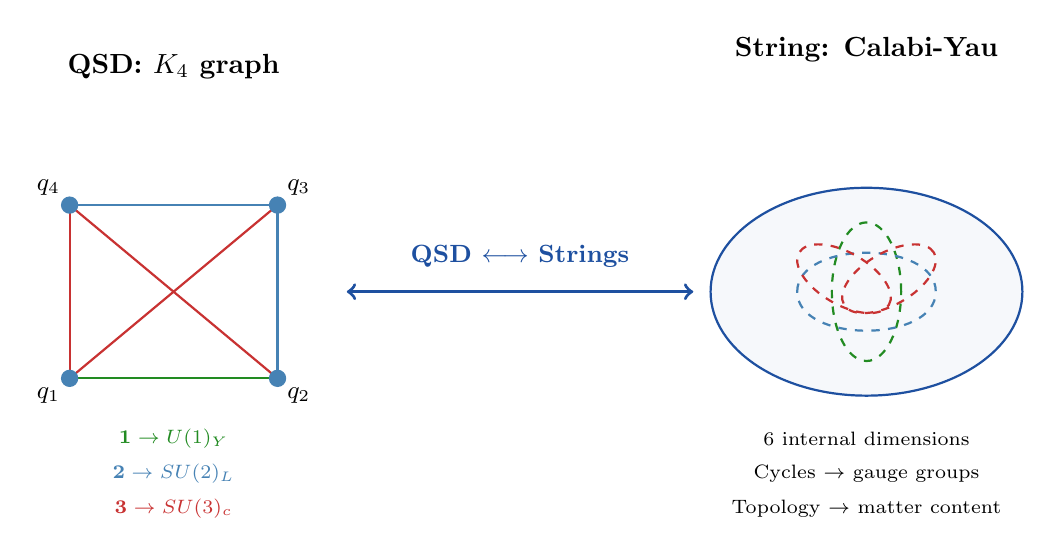
\begin{tikzpicture}[scale=1.1]
    % QSD side (left)
    \begin{scope}[shift={(-4,0)}]
        \node[font=\bfseries] at (0,2.8) {QSD: $K_4$ graph};
        \coordinate (A) at (-1.2,-0.8);
        \coordinate (B) at (1.2,-0.8);
        \coordinate (C) at (1.2,1.2);
        \coordinate (D) at (-1.2,1.2);

        % Edges with color-coding
        \draw[thick, u1color] (A) -- (B);
        \draw[thick, su2color] (B) -- (C);
        \draw[thick, su2color] (C) -- (D);
        \draw[thick, su3color] (D) -- (A);
        \draw[thick, su3color] (A) -- (C);
        \draw[thick, su3color] (B) -- (D);

        % Vertices
        \foreach \p/\lab in {A/$q_1$,B/$q_2$,C/$q_3$,D/$q_4$} {
            \fill[bulkcolor] (\p) circle (0.1);
        }
        \node[font=\small, below left] at (-1.2,-0.8) {$q_1$};
        \node[font=\small, below right] at (1.2,-0.8) {$q_2$};
        \node[font=\small, above right] at (1.2,1.2) {$q_3$};
        \node[font=\small, above left] at (-1.2,1.2) {$q_4$};

        % Legend
        \node[font=\scriptsize, u1color] at (0,-1.5) {$\mathbf{1} \to U(1)_Y$};
        \node[font=\scriptsize, su2color] at (0,-1.9) {$\mathbf{2} \to SU(2)_L$};
        \node[font=\scriptsize, su3color] at (0,-2.3) {$\mathbf{3} \to SU(3)_c$};
    \end{scope}

    % Arrow
    \draw[very thick, <->, stringblue] (-2,0.2) -- (2,0.2)
        node[midway, above, yshift=5pt, font=\small\bfseries] {QSD $\longleftrightarrow$ Strings};

    % String side (right)
    \begin{scope}[shift={(4,0.2)}]
        \node[font=\bfseries] at (0,2.8) {String: Calabi-Yau};

        % Stylized CY manifold
        \draw[thick, stringblue, fill=stringblue!4]
            (0,0) ellipse (1.8 and 1.2);
        % Internal cycles (schematic)
        \draw[thick, u1color, dashed] (0,0) ellipse (0.4 and 0.8);
        \draw[thick, su2color, dashed]
            (-0.8,0) .. controls (-0.8,0.6) and (0.8,0.6) .. (0.8,0)
            .. controls (0.8,-0.6) and (-0.8,-0.6) .. cycle;
        \draw[thick, su3color, dashed, rotate=30]
            (0.3,0) ellipse (0.6 and 0.3);
        \draw[thick, su3color, dashed, rotate=-30]
            (-0.3,0) ellipse (0.6 and 0.3);

        \node[font=\scriptsize] at (0,-1.7) {6 internal dimensions};
        \node[font=\scriptsize] at (0,-2.1) {Cycles $\to$ gauge groups};
        \node[font=\scriptsize] at (0,-2.5) {Topology $\to$ matter content};
    \end{scope}
\end{tikzpicture}
\caption{Gauge group emergence: $K_4$ edge decomposition (left) and Calabi-Yau
cycle wrapping (right) both produce $U(1) \times SU(2) \times SU(3)$.  The
color-coding indicates the correspondence between $S_4$ irreps and cycle
types.}
\label{fig:gauge_correspondence}
\end{figure}

\subsection{Why the Match Is Non-Trivial}

One might object that ``4 + 6 = 10'' is a simple coincidence.  But the
correspondence goes deeper:
\begin{enumerate}[nosep]
    \item The \emph{decomposition} of the 6 internal degrees of freedom
          matches: both produce $1+2+3$ gauge channels.
    \item The \emph{role} of the 4 external degrees matches: both are the
          arena for observable physics.
    \item The \emph{total count of 10} is required by internal consistency
          in both frameworks (quantum anomaly cancellation in strings,
          code perfection in QSD).
\end{enumerate}

\begin{question}[Anomaly Matching]
Does the condition for anomaly-free gauge groups in 10D string compactification
reduce to the $S_4$ decomposition condition when restricted to the $[[5,1,3]]$
code structure?
\end{question}


%==============================================================================
\section{The D-Brane Correspondence}
\label{sec:branes}
%==============================================================================

\subsection{Branes as Physical Objects}

In String Theory, D-branes are not merely mathematical constructs---they
are dynamical objects with mass, charge, and tension.  A D$p$-brane
extends in $p$ spatial dimensions plus time.  Open strings have their
endpoints attached to branes, and the low-energy dynamics of a stack of
$N$ D$p$-branes is a $U(N)$ gauge theory in $(p+1)$ dimensions.

A popular string phenomenology scenario places the Standard Model on a
stack of D3-branes (3 spatial dimensions = our universe) floating in the
10D bulk.  Hidden sectors may live on other, separated branes.

\subsection{The QSD Anchor as a Brane}

In QSD, the Anchor qubit (the 5th qubit of the $[[5,1,3]]$ code) connects
to all 4 bulk qubits and stores the classical record of quantum
processes.  During the ``Snap,'' the anchor decouples from the bulk,
severing 4 bonds and releasing binding energy.

\begin{observation}[Brane Map]
\label{obs:brane}
\begin{align}
\text{Bulk } K_4 \text{ (4 qubits)} &\longleftrightarrow \text{Stack of D3-branes (visible sector)} \\
\text{Anchor qubit ($W$-bit)} &\longleftrightarrow \text{Probe D0-brane (hidden sector)}
\end{align}
\end{observation}

The justification for this identification:
\begin{itemize}[nosep]
    \item The $K_4$ bulk carries gauge symmetry, just as a D3-brane stack
          carries $U(N)$ gauge theory.
    \item The Anchor connects to the bulk via 4 bonds, corresponding to
          open strings stretched between a probe brane and the stack.
    \item The Snap (anchor decoupling) corresponds to brane separation or
          tachyon condensation.
    \item The Ledger (classical record on the anchor) corresponds to the
          D-brane worldvolume theory, which stores information about
          strings that have been absorbed.
\end{itemize}

\begin{figure}[h]
\centering
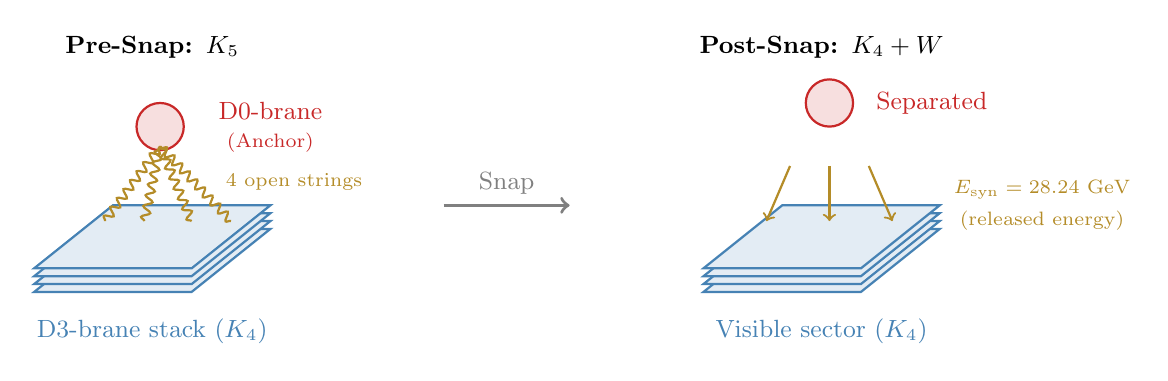
\begin{tikzpicture}[scale=1.0]
    % D3-brane stack (left)
    \begin{scope}[shift={(-3.5,0)}]
        \node[font=\bfseries\small] at (0,3) {Pre-Snap: $K_5$};
        % Brane stack
        \foreach \y in {-0.1,0,0.1,0.2} {
            \draw[thick, bulkcolor, fill=bulkcolor!15]
                (-1.5,\y) -- (-0.5,\y+0.8) -- (1.5,\y+0.8) -- (0.5,\y) -- cycle;
        }
        \node[font=\small, bulkcolor] at (0,-0.6) {D3-brane stack ($K_4$)};

        % Probe brane
        \draw[thick, anchorcolor, fill=anchorcolor!15]
            (0.1,2) circle (0.3);
        \node[font=\small, anchorcolor] at (1.5,2.2) {D0-brane};
        \node[font=\scriptsize, anchorcolor] at (1.5,1.8) {(Anchor)};

        % Stretched strings
        \foreach \x in {-0.8,-0.3,0.3,0.8} {
            \draw[thick, goldenphi, decorate,
                  decoration={snake, amplitude=1.5pt, segment length=4pt}]
                (\x+0.2,0.8) -- (0.1,1.75);
        }
        \node[font=\scriptsize, goldenphi] at (1.8,1.3) {4 open strings};
    \end{scope}

    % Arrow
    \draw[very thick, ->, gray] (0.2,1) -- (1.8,1)
        node[midway, above, font=\small] {Snap};

    % After snap (right)
    \begin{scope}[shift={(5,0)}]
        \node[font=\bfseries\small] at (0,3) {Post-Snap: $K_4 + W$};
        % Brane stack (remains)
        \foreach \y in {-0.1,0,0.1,0.2} {
            \draw[thick, bulkcolor, fill=bulkcolor!15]
                (-1.5,\y) -- (-0.5,\y+0.8) -- (1.5,\y+0.8) -- (0.5,\y) -- cycle;
        }
        \node[font=\small, bulkcolor] at (0,-0.6) {Visible sector ($K_4$)};

        % Separated brane
        \draw[thick, anchorcolor, fill=anchorcolor!15]
            (0.1,2.3) circle (0.3);
        \node[font=\small, anchorcolor] at (1.4,2.3) {Separated};

        % Released energy
        \draw[thick, goldenphi, ->] (-0.4,1.5) -- (-0.7,0.8);
        \draw[thick, goldenphi, ->] (0.1,1.5) -- (0.1,0.8);
        \draw[thick, goldenphi, ->] (0.6,1.5) -- (0.9,0.8);
        \node[font=\scriptsize, goldenphi] at (2.8,1.2) {$\Esyn = 28.24$ GeV};
        \node[font=\scriptsize, goldenphi] at (2.8,0.8) {(released energy)};
    \end{scope}
\end{tikzpicture}
\caption{The Snap mechanism as brane separation.  Left: pre-Snap
configuration with 4 stretched strings connecting the D0-brane (Anchor) to the
D3-stack ($K_4$).  Right: post-Snap, the brane separates and the string energy
is released as the syndrome signal.}
\label{fig:brane_snap}
\end{figure}

\subsection{Brane Processes in QSD Language}

\begin{table}[h]
\centering
\begin{tabular}{p{5.5cm}p{5.5cm}}
\toprule
\textbf{QSD Process} & \textbf{String Theory Process} \\
\midrule
Anchor-bulk coupling ($K_5$ phase) & Open strings stretched between D0 and D3-stack \\[4pt]
Snap (anchor decoupling) & Brane annihilation or tachyon condensation \\[4pt]
Syndrome energy $\Esyn$ & String tension $\times$ brane separation distance \\[4pt]
Ledger (classical record on anchor) & D-brane worldvolume theory \\[4pt]
Infinity bits $\{W,X,Y,Z\}$ & Chan-Paton factors (string endpoint labels) \\[4pt]
Error correction (logical qubit preserved) & Gauge invariance of brane system \\
\bottomrule
\end{tabular}
\caption{Process-level correspondence between QSD dynamics and brane physics.}
\label{tab:brane_processes}
\end{table}

\begin{remark}
The identification of infinity bits with Chan-Paton factors is particularly
suggestive.  In String Theory, Chan-Paton factors are discrete labels attached
to string endpoints on branes, determining which gauge representation a string
state belongs to.  In QSD, infinity bits $\{W,X,Y,Z\}$ are discrete labels
that route information to gauge sectors.  Both are non-dynamical quantum
numbers that organize gauge structure.
\end{remark}

\begin{question}[Chan-Paton Structure]
Do the 4 infinity bits of QSD correspond to specific Chan-Paton assignments in
a D3/D0-brane system?  If so, is the $S_4$ decomposition
$\mathbf{1}\oplus\mathbf{2}\oplus\mathbf{3}$ derivable from the open-string
spectrum?
\end{question}


%==============================================================================
\section{Moduli Stabilization and the Strain $\strain$}
\label{sec:moduli}
%==============================================================================

\subsection{The Central Problem}

In String Theory, the ``moduli problem'' is one of the deepest obstacles
to making contact with observation.  The Calabi-Yau manifold has dozens to
hundreds of moduli---continuous parameters describing its shape and
size---and without a mechanism to fix them, the theory has no predictive
power.

Several mechanisms have been proposed (KKLT~\cite{KKLT2003}, Large Volume Scenario, etc.),
but all require careful tuning.  No mechanism has been shown to uniquely
select the Standard Model vacuum.

\subsection{QSD Stabilization via Code Fidelity}

In QSD, the analog of moduli stabilization is automatic.  The geometric
strain
\begin{equation}
\strain = \frac{3}{80\gr^2} \approx 0.01432
\end{equation}
is not a free parameter to be fixed---it is \emph{derived} from the
requirement that the $K_4$ and $C_5$ graph structures coexist within the
$[[5,1,3]]$ code.  Any other value would break the code's error-correction
capability.

This is analogous to how the geometry of a crystal is fixed by the
requirement that its atoms fit together: there is only one way to tile
them, and that determines all lattice parameters.

\subsection{The Correspondence}

\begin{observation}[Moduli Map]
\label{obs:moduli}
\begin{align}
\text{Geometric strain } \strain &\longleftrightarrow \text{String coupling } \gs
    \text{ (dilaton VEV)} \\
\text{Radion mass } \murad &\longleftrightarrow \text{K\"ahler modulus (volume mode)} \\
\text{Golden ratio } \gr &\longleftrightarrow \text{Complex structure modulus}
\end{align}
\end{observation}

The justification for the $\strain \leftrightarrow \gs$ identification:
\begin{itemize}[nosep]
    \item Both are small dimensionless parameters ($\strain \approx 0.014$;
          $\gs \sim 0.1$ in realistic string vacua).
    \item Both control the strength of quantum corrections: $\strain$
          enters QSD loop corrections as $\strain^n$ at $n$-loop order, just
          as $\gs$ enters string loop corrections as $\gs^{2n}$.
    \item Both must be stabilized for the theory to be predictive.
    \item In QSD, $\strain$ is uniquely fixed by code geometry.  If the
          correspondence holds, this would fix $\gs$ as well, resolving the
          dilaton stabilization problem.
\end{itemize}

\subsection{Vacuum Selection: From $10^{500}$ to 1}

\begin{conjecture}[Vacuum Selection via Error Correction]
\label{conj:vacuum}
The $10^{500}$ string vacua collapse to a unique vacuum under the
requirement that the compactification geometry supports a functioning
quantum error-correcting code.  Specifically:
\begin{equation}
V_{\text{eff}}(\text{moduli}) \propto 1 - \mathcal{F}_{\text{code}}(\text{moduli})
\end{equation}
where $\mathcal{F}_{\text{code}}$ is the fidelity of the $[[5,1,3]]$ code
realized on the compactification geometry.  The universe sits at the unique
minimum where $\mathcal{F}_{\text{code}} = 1$.
\end{conjecture}

The ``Swampland'' (the set of effective field theories that \emph{cannot}
arise from String Theory) would then have a clean characterization~\cite{Vafa2005}: it
consists of all geometries incompatible with perfect quantum error
correction.

\begin{figure}[h]
\centering
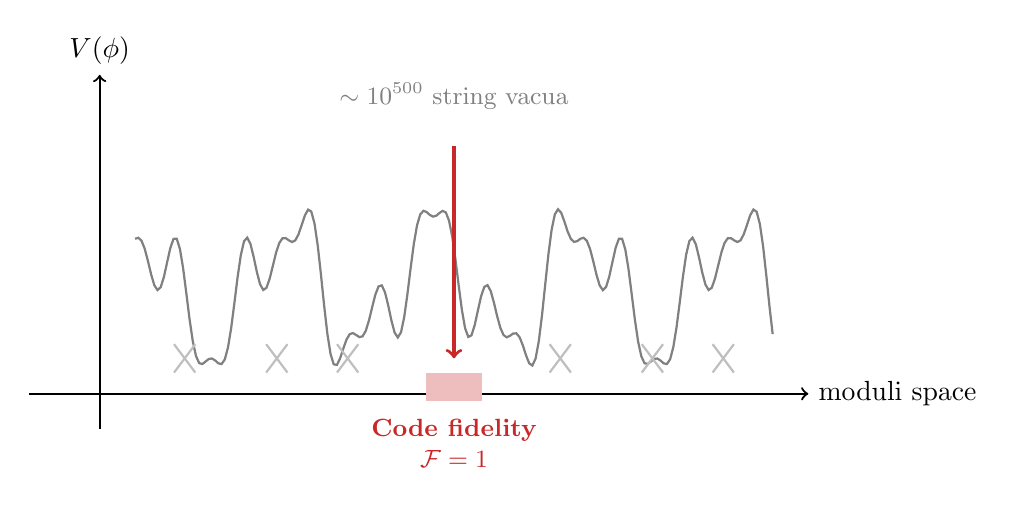
\begin{tikzpicture}[scale=0.9]
    % Landscape
    \draw[thick, ->] (-1,0) -- (10,0) node[right] {moduli space};
    \draw[thick, ->] (0,-0.5) -- (0,4.5) node[above] {$V(\phi)$};

    % Many minima (landscape)
    \draw[thick, gray, domain=0.5:9.5, samples=200]
        plot (\x, {1.5 + 0.8*sin(3*\x r) + 0.5*sin(7*\x r) + 0.3*sin(13*\x r)});

    % Label landscape
    \node[gray, font=\small] at (5,4.2) {$\sim 10^{500}$ string vacua};

    % QSD selection (one minimum highlighted)
    \fill[anchorcolor!30] (4.6,-0.1) rectangle (5.4,0.3);
    \draw[very thick, anchorcolor, ->] (5,3.5) -- (5,0.5);
    \node[anchorcolor, font=\small\bfseries, align=center] at (5,-0.7)
        {Code fidelity\\$\mathcal{F}=1$};

    % Other minima crossed out
    \foreach \x in {1.2, 2.5, 3.5, 6.5, 7.8, 8.8} {
        \draw[thick, gray!50] (\x-0.15,0.3) -- (\x+0.15,0.7);
        \draw[thick, gray!50] (\x-0.15,0.7) -- (\x+0.15,0.3);
    }
\end{tikzpicture}
\caption{Vacuum selection.  The string landscape contains $\sim10^{500}$ local
minima (gray curve).  QSD's code fidelity condition selects a unique vacuum
(red arrow): the one where quantum error correction functions perfectly.}
\label{fig:vacuum_selection}
\end{figure}

\begin{question}[Swampland Correspondence]
Do the known Swampland criteria (Weak Gravity Conjecture, Distance
Conjecture, de~Sitter Conjecture) follow from the requirement that the
vacuum support a $[[5,1,3]]$ code?
\end{question}


%==============================================================================
\section{Renormalization: Topological Finiteness}
\label{sec:renorm}
%==============================================================================

\subsection{The Problem of Infinities}

In standard quantum field theory, loop calculations produce ultraviolet
divergences that must be removed by renormalization.  The procedure works
(spectacularly well in QED), but the loop series is infinite---in
principle, one needs to compute infinitely many diagrams.

Both String Theory and QSD resolve this problem, but through different
(yet structurally parallel) mechanisms.

\subsection{String Theory: Modular Invariance}

String amplitudes are computed as integrals over the moduli space of
Riemann surfaces (the string worldsheet).  At one loop, the worldsheet is
a torus, parametrized by a complex modulus $\tau$.  The key constraint is
\textbf{modular invariance}: the amplitude must be unchanged under
\begin{equation}
\tau \to \tau + 1 \qquad \text{and} \qquad \tau \to -\frac{1}{\tau}
\end{equation}
These transformations map the high-energy region of the integration domain
to the low-energy region, forcing the UV divergences to cancel exactly.

At higher loops, the worldsheet has higher genus (more ``handles''), and
the modular group generalizes.  The result is the same: topology constrains
the integrals and eliminates divergences order by order.

\subsection{QSD: Finite Homology}

QSD renormalization terminates at 3 loops because the graph $K_4 \cup C_5$
has exactly 3 independent topological cycles (first homology group $H_1$).
Each cycle generates one loop correction; after all cycles are exhausted,
no further independent loops can be constructed.

The three corrections and their physical origins (derived in detail in
Supplement~S4):
\begin{align}
\text{1-Loop:} &\quad \delta_1 = +0.239 \quad \text{(network friction: 5 anchor-bulk bonds)} \\
\text{2-Loop:} &\quad \delta_2 = -0.022 \quad \text{(radion feedback via $S_4$ channels)} \\
\text{3-Loop:} &\quad \delta_3 = -0.007 \quad \text{(vacuum drag: zero-point energy)}
\end{align}

Together with the tree-level value $\aem^{-1}_{\text{tree}} = 4\pi\gr^4/\Hbfour
= 136.826$, these yield:
\begin{equation}
\aem^{-1} = 136.826 + 0.239 - 0.022 - 0.007 = 137.036
\end{equation}

\subsection{The Correspondence}

\begin{observation}[Finiteness Map]
\label{obs:finite}
Both frameworks achieve UV finiteness through topology:
\begin{equation}
\text{QSD: finite graph homology} \quad \longleftrightarrow \quad
\text{String: worldsheet modular invariance}
\end{equation}
\end{observation}

\begin{table}[h]
\centering
\begin{tabular}{lcc}
\toprule
\textbf{Loop Order} & \textbf{String Theory} & \textbf{QSD} \\
\midrule
Tree level & Sphere (genus 0) & $K_4$ tree structure \\
1-loop & Torus (genus 1) & Network friction ($+0.239$) \\
2-loop & Double torus (genus 2) & Radion feedback ($-0.022$) \\
3-loop & Triple torus (genus 3) & Vacuum drag ($-0.007$) \\
$\geq$4-loop & Higher genus (suppressed by $\gs^{2n}$) & \textbf{Exactly zero} \\
\bottomrule
\end{tabular}
\caption{Loop structure correspondence.  In String Theory, higher-loop
contributions are suppressed but nonzero.  In QSD, they are exactly zero
because no further independent cycles exist.}
\label{tab:loops}
\end{table}

\begin{remark}[A Stronger Claim?]
QSD's termination is \emph{exact}: there is no 4th loop, period.  String
Theory's higher loops are merely suppressed.  If the duality holds, this
suggests that the higher-genus string contributions, while formally
present, must cancel exactly in the physical vacuum---a testable prediction
within string perturbation theory.
\end{remark}

\begin{figure}[h]
\centering
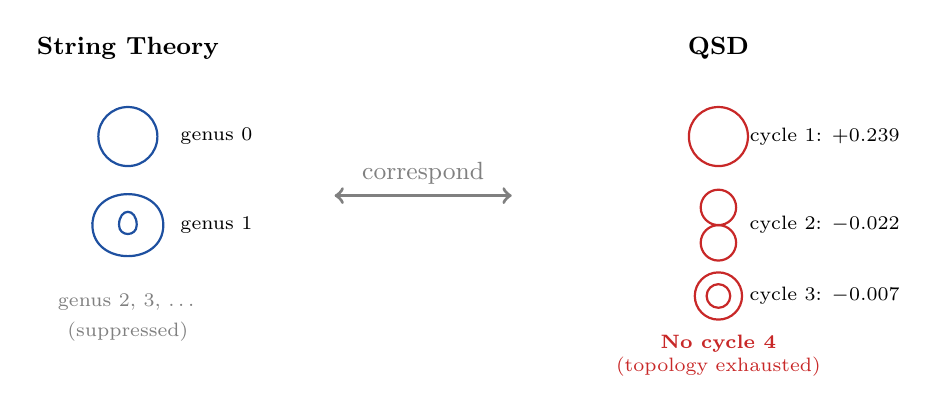
\begin{tikzpicture}[scale=0.75]
    % String side
    \begin{scope}[shift={(-5,0)}]
        \node[font=\bfseries\small] at (0,3.5) {String Theory};
        % Sphere
        \draw[thick, stringblue] (0,2) circle (0.5);
        \node[font=\scriptsize] at (1.5,2) {genus 0};
        % Torus
        \draw[thick, stringblue] (-0.6,0.5) .. controls (-0.6,1.2) and (0.6,1.2) .. (0.6,0.5)
            .. controls (0.6,-0.2) and (-0.6,-0.2) .. cycle;
        \draw[thick, stringblue] (-0.15,0.5) .. controls (-0.15,0.8) and (0.15,0.8) .. (0.15,0.5);
        \draw[thick, stringblue] (-0.15,0.5) .. controls (-0.15,0.3) and (0.15,0.3) .. (0.15,0.5);
        \node[font=\scriptsize] at (1.5,0.5) {genus 1};
        % Higher genus
        \node[font=\scriptsize, gray] at (0,-0.8) {genus 2, 3, \ldots};
        \node[font=\scriptsize, gray] at (0,-1.3) {(suppressed)};
    \end{scope}

    % QSD side
    \begin{scope}[shift={(5,0)}]
        \node[font=\bfseries\small] at (0,3.5) {QSD};
        % Cycle 1
        \draw[thick, anchorcolor] (0,2) circle (0.5);
        \node[font=\scriptsize] at (1.8,2) {cycle 1: $+0.239$};
        % Cycle 2
        \draw[thick, anchorcolor] (0,0.8) circle (0.3);
        \draw[thick, anchorcolor] (0,0.2) circle (0.3);
        \node[font=\scriptsize] at (1.8,0.5) {cycle 2: $-0.022$};
        % Cycle 3
        \draw[thick, anchorcolor] (0,-0.7) circle (0.4);
        \draw[thick, anchorcolor] (0,-0.7) circle (0.2);
        \node[font=\scriptsize] at (1.8,-0.7) {cycle 3: $-0.007$};
        % No cycle 4
        \node[font=\scriptsize\bfseries, anchorcolor] at (0,-1.5) {No cycle 4};
        \node[font=\scriptsize, anchorcolor] at (0,-1.9) {(topology exhausted)};
    \end{scope}

    % Connecting arrow
    \draw[very thick, <->, gray] (-1.5,1) -- (1.5,1)
        node[midway, above, font=\small] {correspond};
\end{tikzpicture}
\caption{Finiteness mechanisms compared.  String Theory achieves UV finiteness
through worldsheet modular invariance at each genus.  QSD achieves exact
termination because the graph $K_4\cup C_5$ has only 3 independent homology
cycles.}
\label{fig:finiteness}
\end{figure}


%==============================================================================
\section{The Hierarchy: Warp Factors and Information Counting}
\label{sec:hierarchy}
%==============================================================================

\subsection{The Problem in Both Frameworks}

Both String Theory and QSD must explain why the electroweak scale
($\sim$100~GeV) is $10^{17}$ times smaller than the Planck scale
($10^{19}$~GeV).  In the Standard Model, this hierarchy requires
fine-tuning to 17 decimal places.

\subsection{String Theory: Warped Compactification}

The Randall-Sundrum (RS) model~\cite{RandallSundrum1999}, originally motivated by string theory,
resolves the hierarchy via a ``warped'' extra dimension.  The metric
takes the form:
\begin{equation}
ds^2 = e^{-2k|y|}\eta_{\mu\nu}dx^\mu dx^\nu + dy^2
\end{equation}
where $k$ is the curvature scale and $y$ parametrizes the extra dimension.
The Planck scale at $y=0$ (the ``UV brane'') is exponentially redshifted
at $y=\pi r$ (the ``IR brane''):
\begin{equation}
\Lambda_{\text{IR}} = e^{-k\pi r}\,\Mpl
\end{equation}
For $k\pi r \approx 37$, this gives $\Lambda_{\text{IR}} \sim 1$~TeV.

\subsection{QSD: Information Reduction}

QSD derives the hierarchy from the state-space volume of the $K_4$
Hilbert space:
\begin{equation}
\murad = \frac{\Mpl}{2^{60}} \times \gr^2 \times (1 - 6\strain) = 25.34~\text{GeV}
\end{equation}
The factor $2^{60} = 16^{15}$ counts the number of distinguishable
micro-configurations per macro-state of the code (see Supplement~S2 for
the full derivation).

\subsection{The Correspondence}

\begin{observation}[Hierarchy Map]
\label{obs:hierarchy}
\begin{equation}
\text{QSD information factor } 2^{-60} \quad \longleftrightarrow \quad
\text{Randall-Sundrum warp factor } e^{-k\pi r}
\end{equation}
\end{observation}

The numerical match: $2^{-60} \approx 8.7 \times 10^{-19}$, while
$e^{-37} \approx 8.5 \times 10^{-17}$.  The two are within two orders of
magnitude, with the remaining difference absorbed by the geometric
factors $\gr^2(1-6\strain)$.

The deeper point is that both mechanisms achieve the hierarchy through
\emph{geometric} or \emph{information-theoretic} counting rather than
fine-tuning.  In the RS model, the warp factor arises from the geometry
of the extra dimension.  In QSD, the factor $2^{-60}$ arises from the
combinatorics of the code.

\subsection{T-Duality and UV/IR Mixing}

String Theory possesses a remarkable symmetry called \textbf{T-duality}: a
compactified dimension of radius $R$ is physically identical to one of
radius $\ap/R$~\cite{Polchinski1998v1}.  This implies a minimum observable length
$L_{\text{min}} \sim \sqrt{\ap} = \ls$ and connects ultraviolet (small
distance) physics to infrared (large distance) physics.

QSD exhibits an analogous structure.  The Ledger mechanism stores
high-energy information (entering a horizon) as low-energy bits on the
boundary.  The hierarchy is the necessary consequence of this
encoding---the conversion factor between ``UV bits'' (Planck-scale data)
and ``IR bits'' (electroweak-scale observables) is precisely $2^{60}$.

\begin{question}[T-Duality Analog]
Is there a precise QSD analog of T-duality---a symmetry that exchanges the
$K_4$ (``internal'') and $C_5$ (``external'') graph structures while
preserving the physics?
\end{question}


%==============================================================================
\section{The 28 GeV Anomaly in String Language}
\label{sec:anomaly}
%==============================================================================

\subsection{QSD Prediction}

QSD predicts a syndrome signature at:
\begin{equation}
\Esyn = \murad(1 + 8\strain) = 25.34 \times 1.1146 = 28.24~\text{GeV}
\end{equation}
matching the CMS dimuon excess at $\sim28.3$~GeV to 0.2\% (see
Supplement~S5 for the complete phenomenological analysis).

\subsection{Three String-Theoretic Interpretations}

The 28~GeV signal admits at least three natural interpretations in string
language:

\paragraph{(a) The Breathing Mode / Radion.}
In Calabi-Yau compactification, the overall volume of the internal
manifold can oscillate.  The quantum of this oscillation---the
``breathing mode'' or radion---is a scalar field whose mass is set by the
stabilization potential.  In QSD, the radion mass is
$\murad = 25.34$~GeV; the syndrome energy $\Esyn = 28.24$~GeV includes
the binding energy of anchor-bulk bonds.

\paragraph{(b) The Lightest Kaluza-Klein Mode.}
In theories with extra dimensions, every 4D field has a tower of
``Kaluza-Klein'' (KK) excitations---higher harmonics on the compactified
dimensions.  In warped scenarios, the lightest KK mode is brought from
the Planck scale to the electroweak scale by the warp factor.  The QSD
hierarchy formula naturally produces this mode at $\sim 25$~GeV.

\paragraph{(c) A Stretched String.}
In the brane picture, a string momentarily stretched between the visible
sector (D3-stack) and the hidden sector (D0/Anchor) would have energy
proportional to the brane separation times the string tension.  The
syndrome is the energy released when this string snaps.

\subsection{Why It Couples Preferentially to $b$-Quarks}

In warped geometries (Randall-Sundrum), the 5D wavefunctions of Standard
Model fermions are localized at different positions along the extra
dimension.  Heavy fermions (top, bottom) are localized near the IR
brane, while light fermions (electron, up-quark) are localized near the
UV brane.

The radion field also lives on the IR brane.  Therefore:
\begin{equation}
\text{Coupling}(\text{radion}, f) \propto
    |\Psi_f(y_{\text{IR}})|^2 \propto m_f
\end{equation}
Heavy quarks have large wavefunction overlap with the radion; light leptons
have small overlap.  This is precisely the mass-proportional coupling
derived in QSD from the radion-matter Lagrangian:
\begin{equation}
\LL_{\text{int}} = -\frac{\phi_r}{v_r}\sum_f m_f\bar\psi_f\psi_f
\end{equation}

\subsection{Why the Signal Saturates}

The QSD prediction that the syndrome significance \emph{saturates} (stops
growing with luminosity) has a natural holographic interpretation.

In AdS/CFT, a bulk particle corresponds to a boundary operator~\cite{Maldacena1999,Almheiri2015}.  The production rate of bulk excitations is limited by the \textbf{information-processing capacity} of the holographic boundary---the Ledger.  You cannot create radion excitations faster than the Ledger can record them.

This is analogous to the Bekenstein bound: there is a maximum amount of
information that can be processed per unit area per unit time.  The
syndrome production rate is bounded by this information bandwidth.

\textbf{String verdict}: The saturation, if confirmed by LHC Run~3, would
be evidence of the holographic principle at collider energies---a
genuinely novel signature.


%==============================================================================
\section{The Complete Dictionary}
\label{sec:dictionary}
%==============================================================================

We collect all correspondences identified in the preceding sections into a
single reference table.

\begin{table}[h]
\centering
\small
\begin{tabular}{p{5.8cm}p{5.8cm}}
\toprule
\textbf{QSD Concept} & \textbf{String Theory Analog} \\
\midrule
\multicolumn{2}{l}{\textit{Structure}} \\
$K_4$ nodes (4) & Spacetime dimensions (4) \\
$K_4$ edges (6) & Calabi-Yau dimensions (6) \\
$S_4$ edge decomposition $\mathbf{1}\oplus\mathbf{2}\oplus\mathbf{3}$ & Gauge groups from CY cycles \\
Anchor qubit ($W$-bit) & D0-brane / probe brane \\
Bulk $K_4$ & D3-brane stack \\
Infinity bits $\{W,X,Y,Z\}$ & Chan-Paton factors \\
$C_5$ cyclic symmetry ($\mathbb{Z}_5$) & Orbifold symmetry \\
\midrule
\multicolumn{2}{l}{\textit{Parameters}} \\
Geometric strain $\strain$ & String coupling $\gs$ / dilaton VEV \\
Radion mass $\murad$ & K\"ahler modulus (volume mode) \\
Golden ratio $\gr$ & Complex structure modulus \\
$\Hbfour = 1/(4\ln 2)$ & String tension $\ap$ (related) \\
$\Hbfour/\strain$ (holographic bit density / strain) & Dilaton / K\"ahler ratio \\
\midrule
\multicolumn{2}{l}{\textit{Mechanisms}} \\
Snap mechanism & Brane separation / tachyon condensation \\
Syndrome energy 28.24 GeV & Lightest KK mode / stabilized radion \\
3-loop termination & Modular invariance \\
Hierarchy factor $2^{-60}$ & Warp factor $e^{-k\pi r}$ \\
Code stability condition & Swampland constraints \\
Signal saturation & Holographic bandwidth limit \\
$[[5,1,3]]$ error correction & Gauge invariance preservation \\
Logical qubit (Higgs) & Lightest string mode \\
\bottomrule
\end{tabular}
\caption{Complete QSD--String Theory dictionary.  Structural elements,
parameters, and dynamical mechanisms are matched across frameworks.}
\label{tab:full_dictionary}
\end{table}


%==============================================================================
\section{Strategic Implications}
\label{sec:strategy}
%==============================================================================

If the correspondence identified above proves to be a genuine duality, both
frameworks gain significantly.

\subsection{What QSD Provides to String Theory}

\begin{enumerate}
    \item \textbf{Vacuum Selection.}  The code fidelity condition
          (Conjecture~\ref{conj:vacuum}) picks one vacuum from $10^{500}$.
          This would resolve the Landscape problem that has stymied string
          phenomenology for two decades.

    \item \textbf{Predictive Power.}  QSD derives $\aem^{-1} = 137.036$,
          $\sin^2\theta_W = 0.2312$, $\mH = 126.7$~GeV---values that
          String Theory currently takes as input.  A duality would mean
          String Theory \emph{predicts} these values via QSD.

    \item \textbf{A Testable Low-Energy Prediction.}  The 28~GeV syndrome
          gives String Theory its first prediction below the Planck scale
          that is accessible to current experiments.

    \item \textbf{The Target Manifold.}  If QSD is correct, string
          theorists should look for a Calabi-Yau with Euler
          characteristic $|\chi| = 6$ (since $|\chi|/2 = 3$ generations).
          This dramatically narrows the search within the Kreuzer-Skarke
          database~\cite{KreuzerSkarke2000}.
\end{enumerate}

\subsection{What String Theory Provides to QSD}

\begin{enumerate}
    \item \textbf{Mathematical Rigor.}  String Field Theory provides
          formal tools for the Snap mechanism (brane dynamics, tachyon
          condensation, open-string field theory).

    \item \textbf{Conceptual Validation.}  T-duality justifies the
          existence of a minimum length scale; modular invariance justifies
          finite loop corrections.  These are established results in String
          Theory that would bolster QSD's claims.

    \item \textbf{Community and Credibility.}  Framing QSD as ``the
          non-perturbative vacuum of String Theory'' connects it to an
          established research program with thousands of practitioners,
          removing the ``radical outsider'' label.

    \item \textbf{Gravitational Extension.}  String Theory naturally
          includes gravity; QSD currently addresses only particle physics.
          The duality could provide QSD's gravitational sector ``for
          free.''
\end{enumerate}

\subsection{The Duality Conjecture}

\begin{conjecture}[QSD--String Duality]
\label{conj:duality}
Quantum Spectrodynamics is to String Theory as Matrix Theory~\cite{BFSS1997} is to M-Theory: a discrete, non-perturbative definition of the vacuum state that the continuum theory describes perturbatively.

Specifically: there exists a Calabi-Yau threefold $X$ with $\chi(X) = \pm 6$
such that the Type~IIB string compactification on $X$ with appropriate
flux configuration reproduces all QSD predictions in the low-energy limit.
\end{conjecture}

\begin{remark}
The Matrix Theory analogy is deliberate.  Matrix Theory
provides a non-perturbative definition of M-Theory using a discrete
quantum-mechanical system (a matrix model).  It was discovered by
computing quantities in both frameworks and finding agreement.  We propose
the same investigative strategy for QSD and String Theory.
\end{remark}


%==============================================================================
\section{Open Questions and Research Program}
\label{sec:questions}
%==============================================================================

We close with a structured list of open questions, organized by the
expertise required to address them.

\subsection{For String Theorists}

\begin{question}[Calabi-Yau Search]
Does the Kreuzer-Skarke database~\cite{KreuzerSkarke2000} contain a Calabi-Yau threefold with
$|\chi| = 6$ whose intersection numbers reproduce the $S_4$ decomposition
$\mathbf{1}\oplus\mathbf{2}\oplus\mathbf{3}$?
\end{question}

\begin{question}[Modular Invariance Implies Termination?]
In the physical vacuum (if it corresponds to QSD), do the genus $\geq 4$
string amplitudes cancel exactly, or are they merely suppressed?
\end{question}

\begin{question}[KKLT and Code Fidelity]
Can the KKLT moduli stabilization mechanism~\cite{KKLT2003} be reformulated as a
code-fidelity maximization problem?  Does the resulting potential have a
unique minimum?
\end{question}

\subsection{For Quantum Information Theorists}

\begin{question}[Code from Geometry]
Can the $[[5,1,3]]$ code be derived from a Calabi-Yau compactification, or
more generally, can quantum error-correcting codes be classified by the
topology of their ``parent'' manifolds?
\end{question}

\begin{question}[Holographic Codes]
Is the $[[5,1,3]]$ code a special case of holographic tensor network codes
(e.g., HaPPY codes)?  If so, what is the corresponding bulk geometry?
\end{question}

\subsection{For Phenomenologists}

\begin{question}[KK Tower]
If the 28~GeV signal is the lightest KK mode, where are the heavier modes?
QSD predicts the next syndrome at $\sim\murad(1 + 16\strain^2) \approx
25.4$~GeV (two-qubit error), but this may not be observable.  What are the
signatures of the KK tower in the QSD/string picture?
\end{question}

\begin{question}[Proton Decay Channel]
QSD predicts $\tau_p \sim 10^{38-40}$~years from code distance.  String
Theory predicts proton decay via dimension-6 operators with
model-dependent rates.  Do the two predictions agree for the candidate
Calabi-Yau?
\end{question}


%==============================================================================
\section{Conclusion: An Invitation}
\label{sec:conclusion}
%==============================================================================

This supplement does not claim to derive String Theory results.  The
author is an information theorist, not a string theorist.

What we have shown is a \textbf{structural isomorphism}: the same numbers
(4 external, 6 internal), the same finiteness mechanism (topology), the
same hierarchy ($10^{17}$), and the same energy scale ($\sim25$~GeV)
appear in both frameworks.  The correspondence extends to dynamics (Snap
$\leftrightarrow$ brane separation), parameters ($\strain \leftrightarrow
\gs$), and even phenomenology (mass-proportional coupling from IR brane
localization).

We invite the string theory community to investigate:
\begin{enumerate}
    \item Can the $[[5,1,3]]$ code be derived from a specific Calabi-Yau
          compactification?
    \item Does the code stability condition correspond to known Swampland
          criteria?
    \item Can String Field Theory calculate the syndrome production
          cross-section?
    \item Is there a Calabi-Yau with $|\chi| = 6$ that reproduces QSD's
          predictions?
\end{enumerate}

If the correspondence holds, QSD provides what String Theory has sought
for 40 years: \textbf{the principle that selects the Standard Model from
the Landscape.}

And if it does not hold, the specific points of failure will sharpen
both frameworks.

%==============================================================================
% REFERENCES
%==============================================================================

\bibliographystyle{unsrt}
\bibliography{qsd_references}

\end{document}
